% ------------------------------------------------------------------------------
% TYPO3 Version 10.2 - What's New (English Version)
%
% @author	Michael Schams <schams.net>
% @license	Creative Commons BY-NC-SA 3.0
% @link		https://typo3.org/help/documentation/whats-new/
% @language	English
% ------------------------------------------------------------------------------

\section{Introduction}
\begin{frame}[fragile]
	\frametitle{Introduction}

	\begin{center}\huge{Introduction}\end{center}
	\begin{center}\huge{\color{typo3darkgrey}\textbf{The Facts}}\end{center}

\end{frame}

% ------------------------------------------------------------------------------
% TYPO3 Version 10.2 - The Facts

\begin{frame}[fragile]
	\frametitle{Introduction}
	\framesubtitle{TYPO3 Version 10.2 - The Facts}

	\begin{itemize}
		\item Release date: 03 December 2019
		\item Release type: Sprint Release
	\end{itemize}

	\begin{figure}
		
\includegraphics[width=0.95\linewidth]{Introduction/typo3-v10-2-banner.png}
	\end{figure}

\end{frame}

% ------------------------------------------------------------------------------
% TYPO3 Version 10.2 - Executive Summary

\begin{frame}[fragile]
	\frametitle{Introduction}
	\framesubtitle{Executive Summary}

	\small
		TYPO3 version 10.2 is the third sprint release on the way to the LTS-version
		(long-term support) in 2020. It is also the last sprint release of the year.

		\vspace{0.2cm}

		A lot of functionality was developed during the TYPO3 Initiative Week (T3INIT19)
		and TYPO3 v10.2 already contains some of these components.

		\vspace{0.2cm}

		This release paves the way for a cutting-edge environment. TYPO3 v10.2 not only
		supports Symfony version 5.0, but is also the first TYPO3 release that supports
		PHP version 7.4. It also marks the last release before the feature freeze release
		in February 2020.

	\normalsize

\end{frame}

% ------------------------------------------------------------------------------
% System Requirements

\begin{frame}[fragile]
	\frametitle{Introduction}
	\framesubtitle{System Requirements}

	\begin{itemize}
		\item PHP version 7.2, 7.3 or 7.4
		\item PHP settings:

			\begin{itemize}
				\item \texttt{memory\_limit} >= 256M
				\item \texttt{max\_execution\_time} >= 240s
				\item \texttt{max\_input\_vars} >= 1500
				\item compilation option \texttt{-}\texttt{-disable-ipv6} must \underline{not} be used
			\end{itemize}

		\item Most database servers supported by \textbf{Doctrine DBAL} also work with TYPO3.
			Tested DB engines are for example:
	\end{itemize}

	\begin{figure}
		
\includegraphics[width=0.80\linewidth]{Introduction/logo-databases.png}
	\end{figure}

\end{frame}

% ------------------------------------------------------------------------------
% Development, Release and Maintenance Timeline

\begin{frame}[fragile]
	\frametitle{Introduction}
	\framesubtitle{Development, Release and Maintenance Timeline}

	\textbf{TYPO3 v10}

	\begin{figure}
		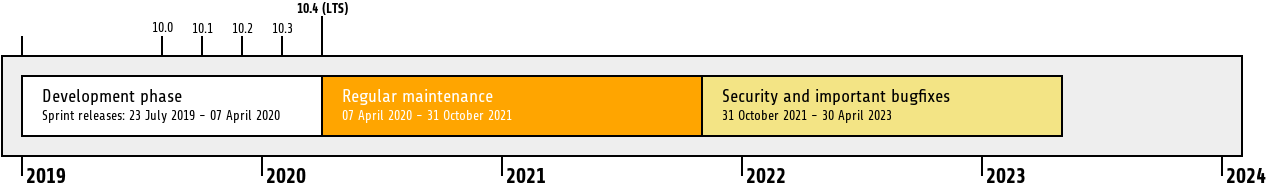
\includegraphics[width=1\linewidth]{Introduction/typo3-v10-lifecycle.png}
	\end{figure}

	\textbf{Extended Support}\newline
	\smaller
		The \href{https://typo3.com}{TYPO3 GmbH} offers further support options
		for TYPO3 v10 LTS even after 30 April 2023 for up to two additional
		years.
	\normalsize

\end{frame}

% ------------------------------------------------------------------------------
% TYPO3 v10 Roadmap

\begin{frame}[fragile]
	\frametitle{Introduction}
	\framesubtitle{TYPO3 v10 Roadmap}

	Release dates and their primary focus:

	\begin{itemize}

		\item v10.0 \tabto{1.1cm}23/July/2019\tabto{3.4cm}Pave the way for exciting new concepts and APIs
		\item v10.1 \tabto{1.1cm}01/Oct/2019\tabto{3.4cm}Routing Improvements and Site Handling v2
		\item
			\begingroup
				\color{typo3orange}
				v10.2 \tabto{1.1cm}03/Dec/2019\tabto{3.4cm}Fluid/Rendering Engine Improvements
			\endgroup
		\item v10.3 \tabto{1.1cm}04/Feb/2020\tabto{3.4cm}Feature Freeze
		\item v10.4 \tabto{1.1cm}07/Apr/2020\tabto{3.4cm}LTS Release (Long-term Support)

	\end{itemize}

	\smaller
		\url{https://typo3.org/article/typo3-v10-roadmap/}\newline
		\url{https://typo3.org/article/typo3-v10-safe-and-sound/}
	\normalsize

\end{frame}

% ------------------------------------------------------------------------------
% Installation

\begin{frame}[fragile]
	\frametitle{Introduction}
	\framesubtitle{Installation}

	\begin{itemize}
		\item Official \textit{classic} installation procedure under Linux/Mac OS X\newline
			(DocumentRoot for example \texttt{/var/www/site/htdocs}):
\begin{lstlisting}
$ cd /var/www/site
$ wget --content-disposition get.typo3.org/10.2
$ tar xzf typo3_src-10.2.0.tar.gz
$ cd htdocs
$ ln -s ../typo3_src-10.2.0 typo3_src
$ ln -s typo3_src/index.php
$ ln -s typo3_src/typo3
$ touch FIRST_INSTALL
\end{lstlisting}

		\item Symbolic links under Microsoft Windows:

			\begin{itemize}
				\item Use \texttt{junction} under Windows XP/2000
				\item Use \texttt{mklink} under Windows Vista and Windows 7 and higher
			\end{itemize}

	\end{itemize}
\end{frame}

% ------------------------------------------------------------------------------
% Installation using composer

\begin{frame}[fragile]
	\frametitle{Installation and Upgrade}
	\framesubtitle{Installation Using \texttt{composer}}

	\begin{itemize}
		\item Installation using \textit{composer} under Linux, Mac OS X and Windows 10:
\begin{lstlisting}
$ cd /var/www/site/
$ composer create-project typo3/cms-base-distribution typo3v10 ^10.2
\end{lstlisting}

		\item Alternatively, create your custom \texttt{composer.json} file and run:
\begin{lstlisting}
$ composer install
\end{lstlisting}

			Further details and examples for \texttt{composer.json} files are available at:\newline
			\smaller
				\href{https://composer.typo3.org}{https://composer.typo3.org}
			\normalsize

	\end{itemize}
\end{frame}

% ------------------------------------------------------------------------------
